\begin{figure}[H]
    \captionsetup[subfigure]{labelformat=empty}
    \begin{subfigure}[t]{0.47\textwidth}
        \begin{subfigure}[t]{0.49\textwidth}
            \caption{A}
            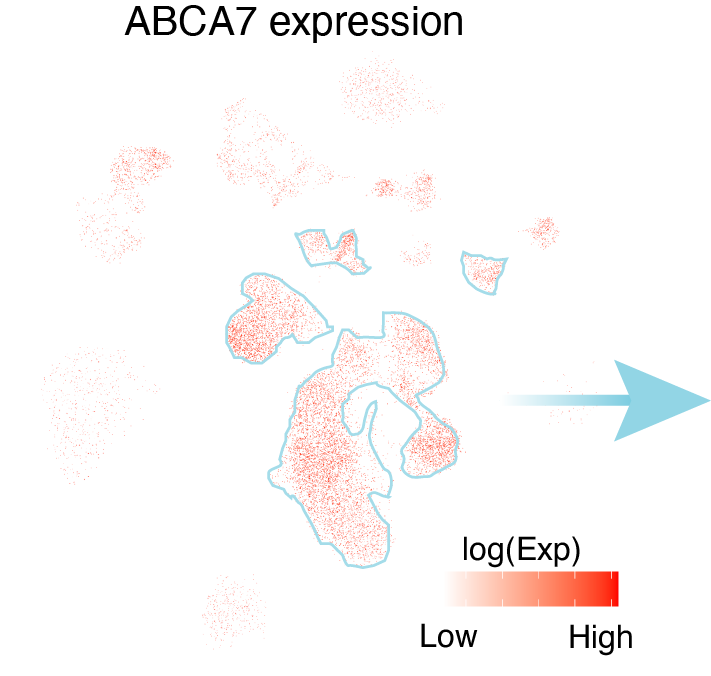
\includegraphics[width=\textwidth]{./main_plots/cell_projection_abca7_expression.png}        
        \end{subfigure}
        \begin{subfigure}[t]{0.49\textwidth}
            %\caption{}
            \vspace{1cm}
            \includegraphics[width=\textwidth]{./main_plots/pm_kl_network_network.pdf}        
        \end{subfigure}
        \begin{subfigure}[t]{\textwidth}
            \caption{C}
            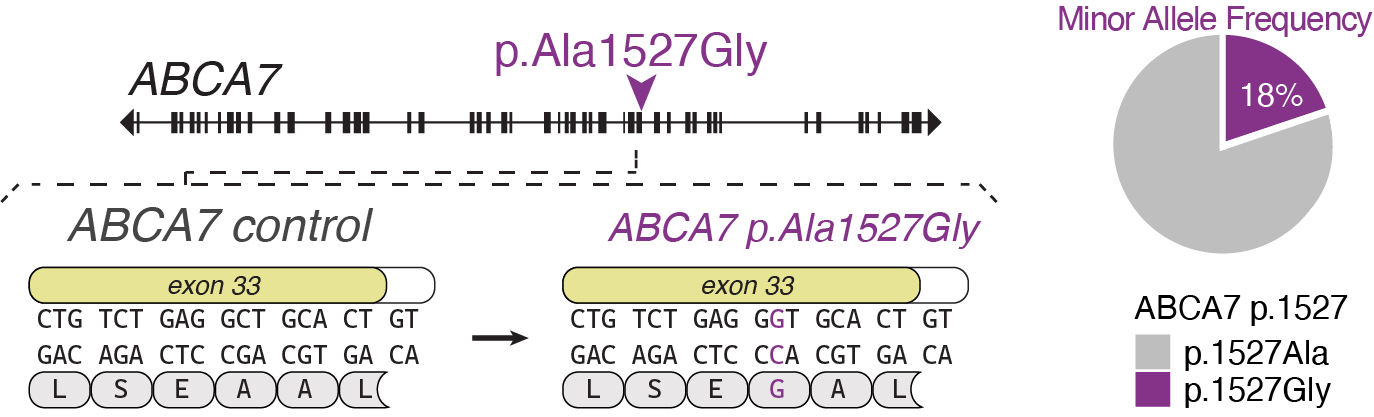
\includegraphics[width=\textwidth]{./main_plots/common_variant_cartoon.png}        
        \end{subfigure}
    \end{subfigure}
    \begin{subfigure}[t]{0.45\textwidth}
        \caption{B}
        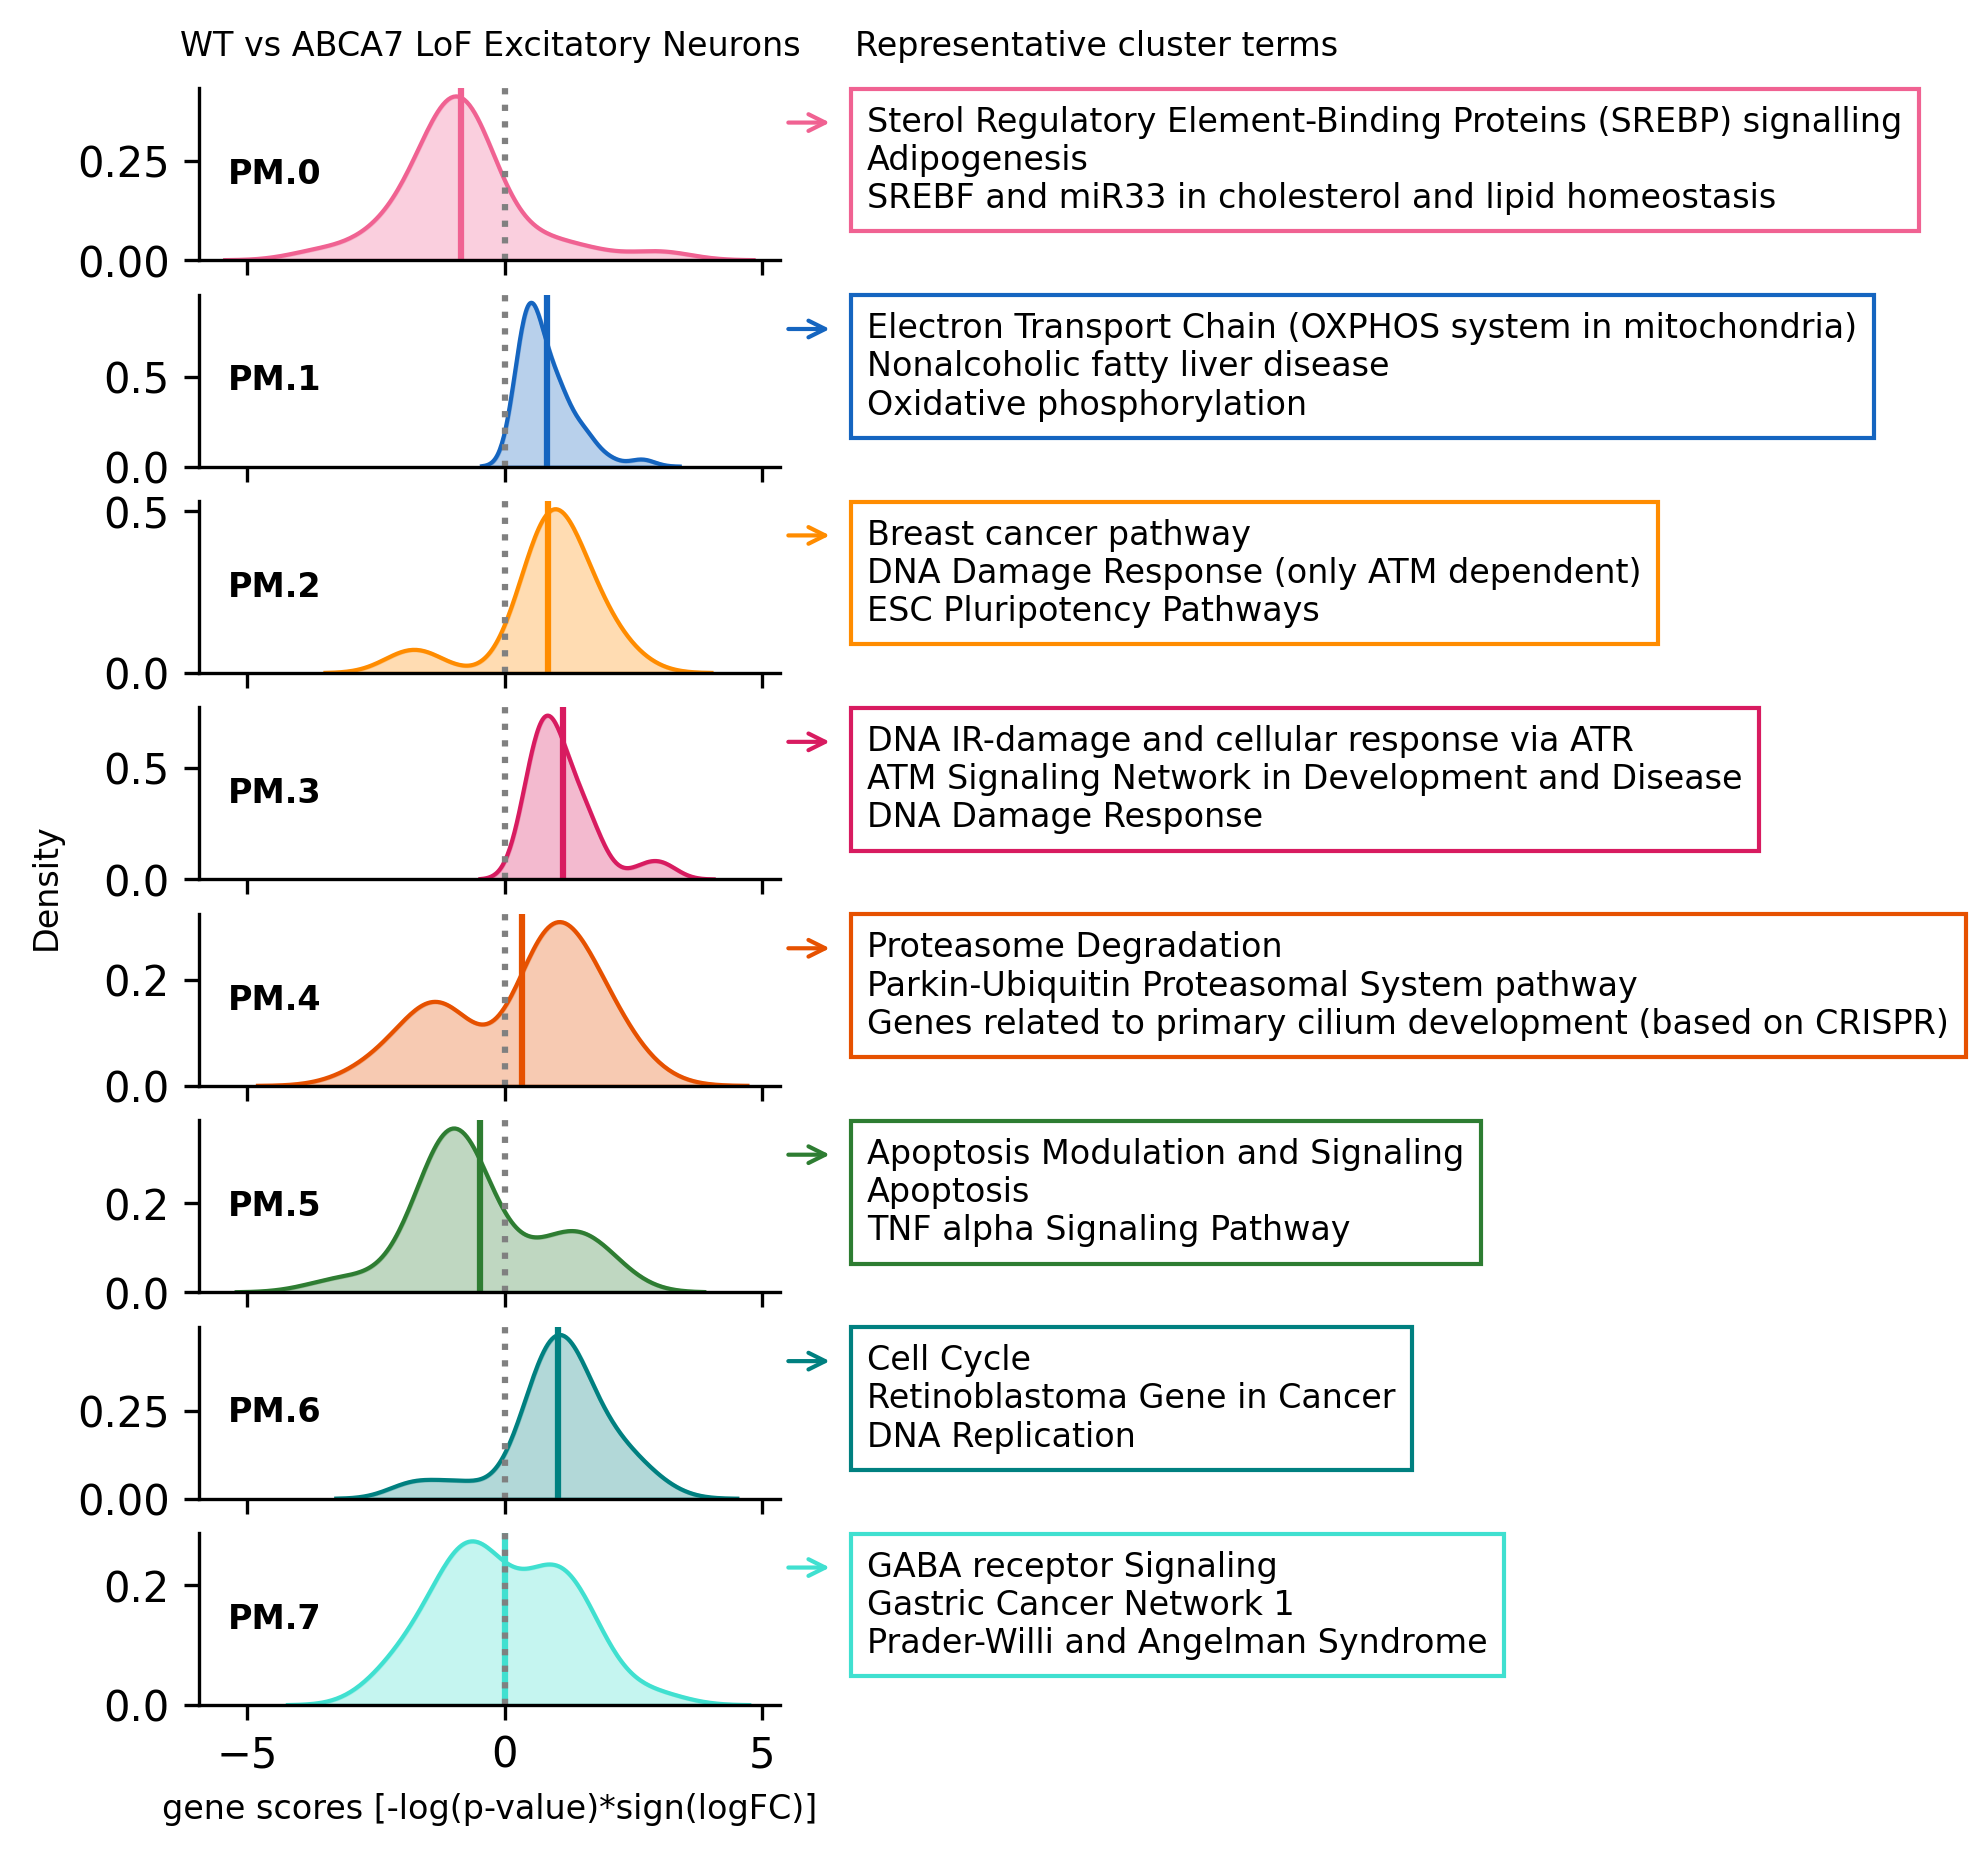
\includegraphics[width=\textwidth]{./main_plots/kl_densities.png}        
    \end{subfigure}
    \begin{subfigure}[t]{0.3\textwidth}
        \caption{E}
        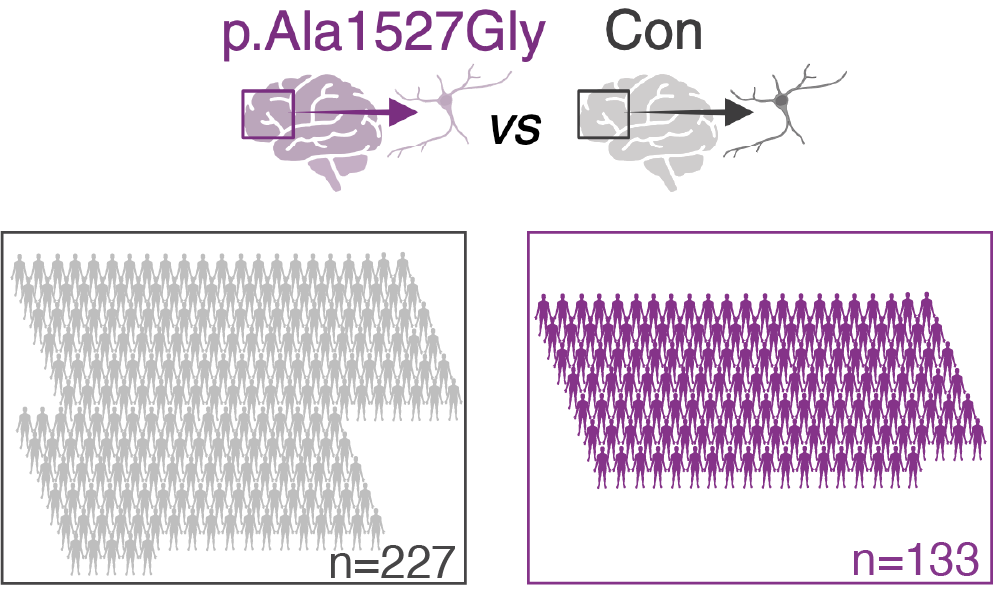
\includegraphics[width=\textwidth]{./main_plots/common_var_cohort_cartoon.png}        
    \end{subfigure}
    \hspace{0.01\textwidth} % Adjust this value as needed
    \begin{subfigure}[t]{0.225\textwidth}
        \caption{F}
        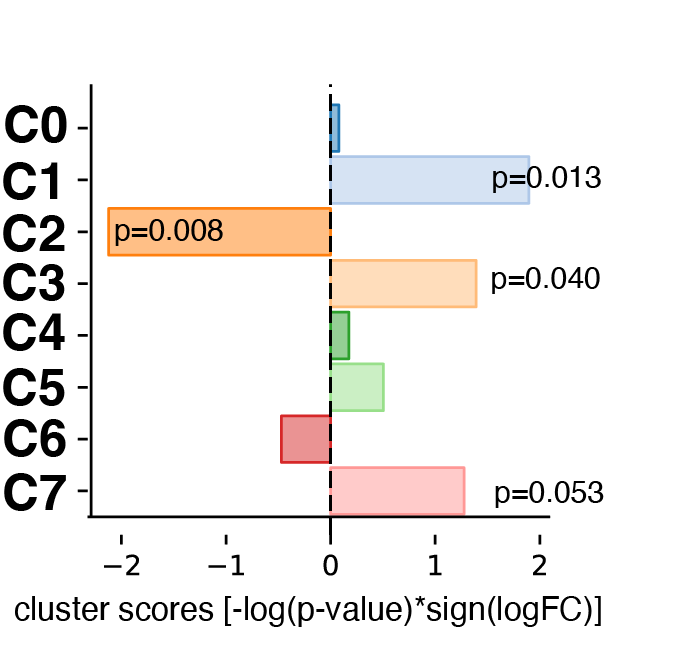
\includegraphics[width=\textwidth]{./main_plots/variant_path_scores.png}        
    \end{subfigure}
    \begin{subfigure}[t]{0.45\textwidth}
        \caption{G}
        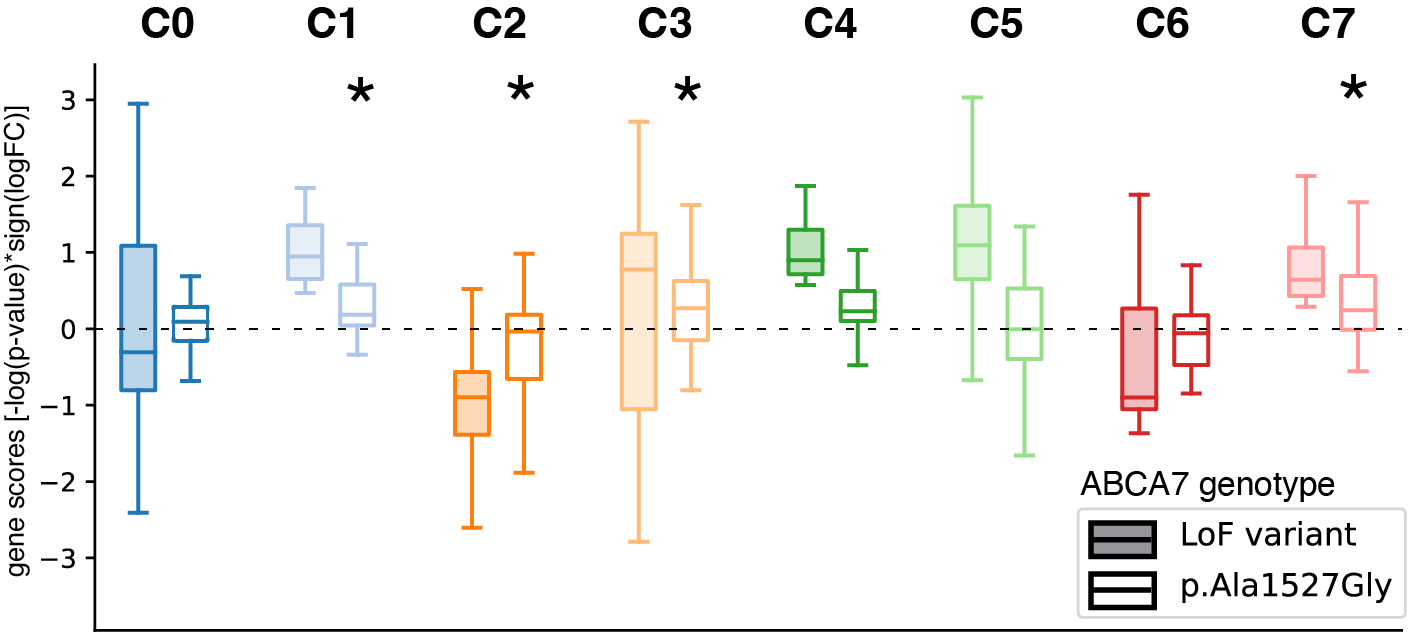
\includegraphics[width=\textwidth]{./main_plots/common_var_distributions.png}        
    \end{subfigure}
    \begin{subfigure}[t]{0.3\textwidth}
        \caption{H}
        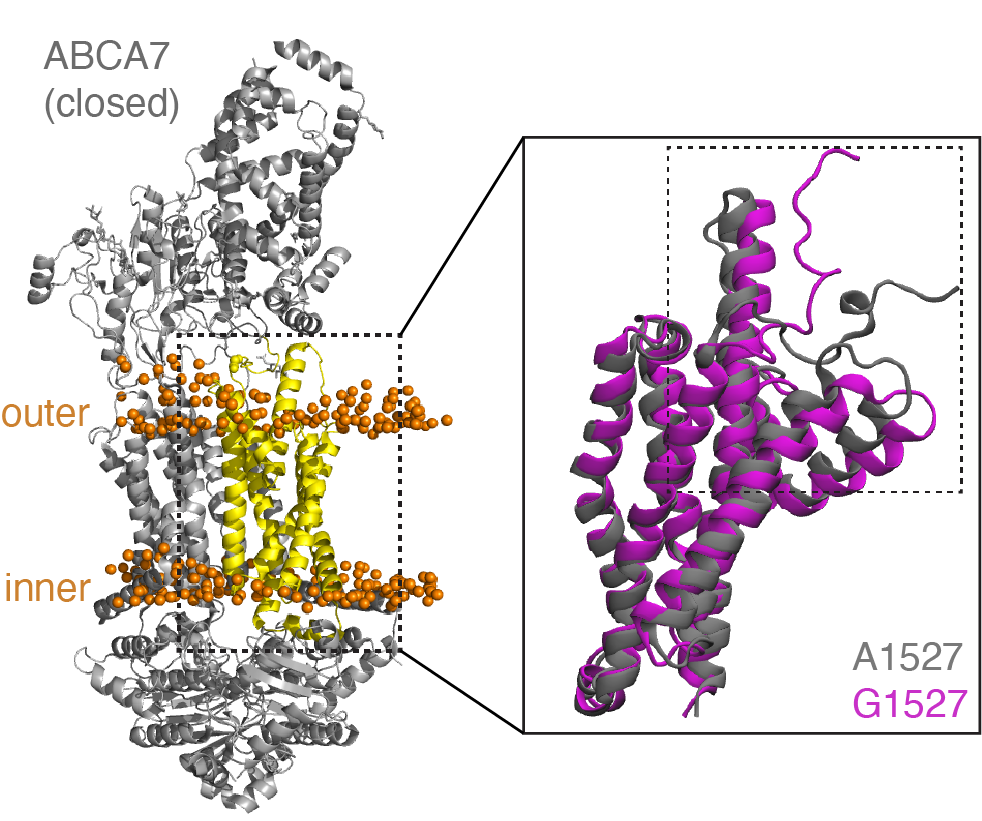
\includegraphics[width=\textwidth]{./main_plots/abca7_structure_with_inset.png}        
    \end{subfigure}
    \begin{subfigure}[t]{0.165\textwidth}
        \caption{I}
        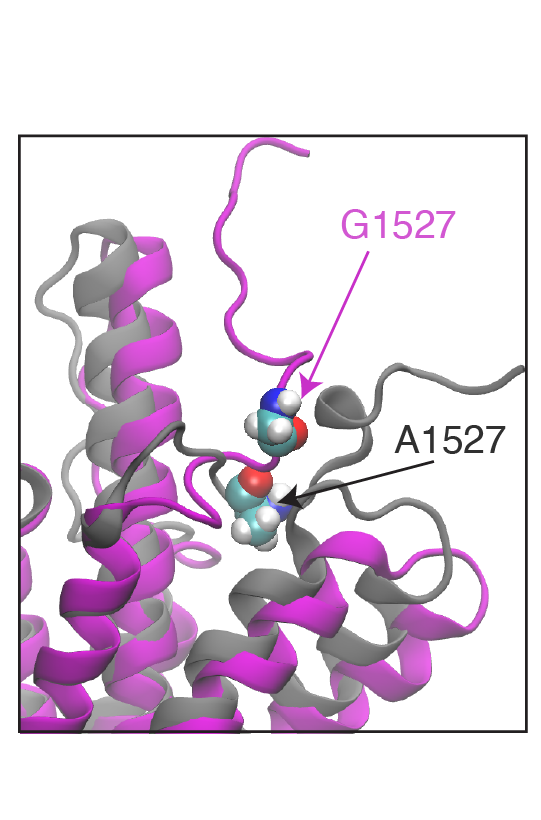
\includegraphics[width=\textwidth]{./main_plots/abca7_inset_only.png}        
    \end{subfigure}
    \hspace{0.01\textwidth} % Adjust this value as needed
    \begin{subfigure}[t]{0.32\textwidth}
        \caption{J}
        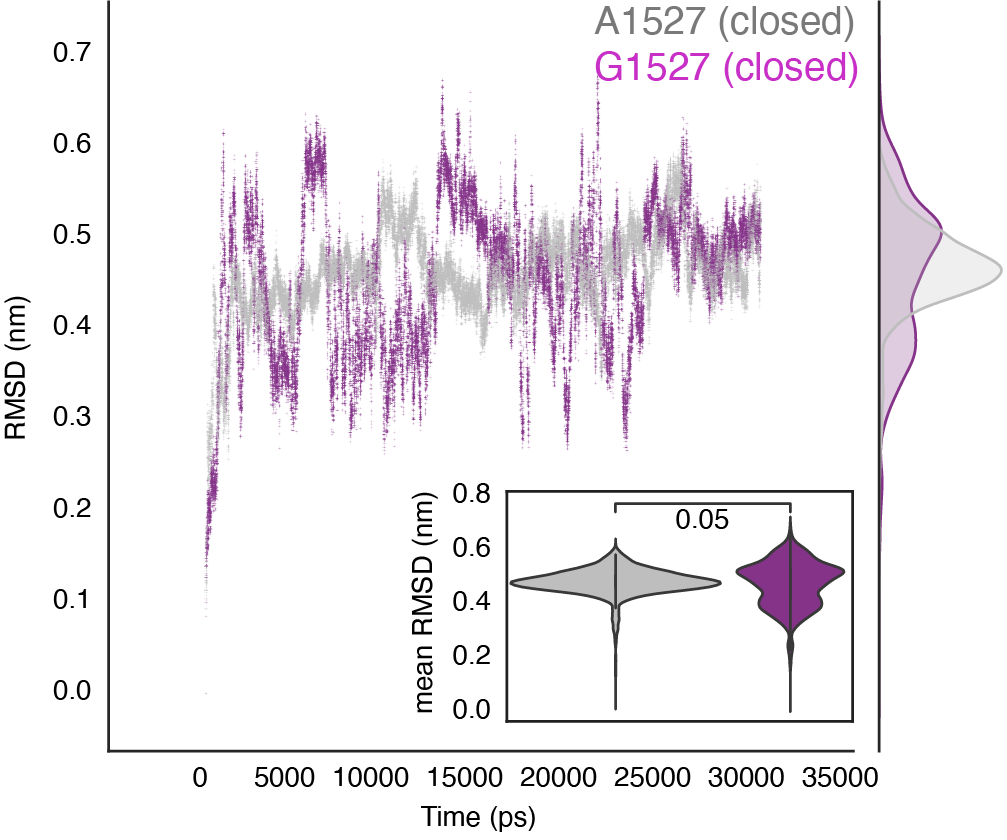
\includegraphics[width=\textwidth]{./main_plots/variant_dynamics.png}        
    \end{subfigure}
    \begin{subfigure}[t]{0.16\textwidth}
        \caption{K}
        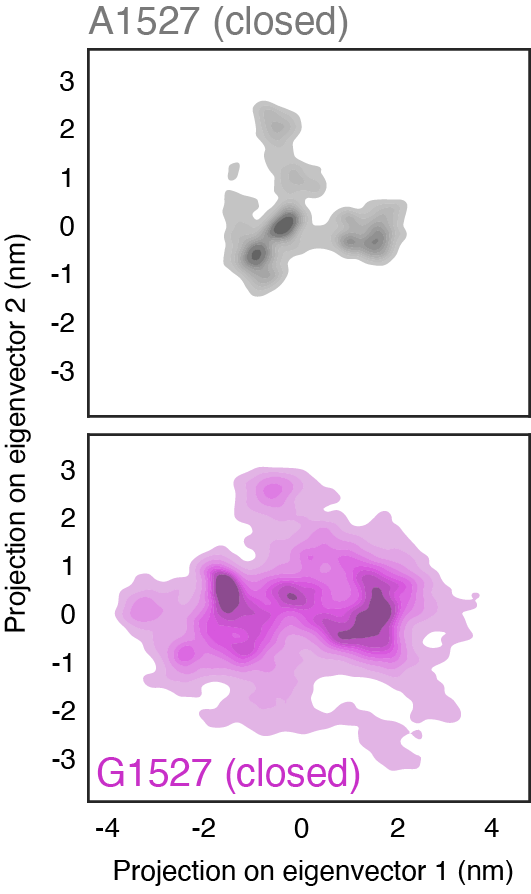
\includegraphics[width=\textwidth]{./main_plots/variant_projection_closed.png}        
    \end{subfigure}
    \caption{
        \textbf{Transcriptional Perturbations in Excitatory Neurons in ABCA7 LoF and ABCA7 p.Ala1527Gly Variant Carriers.}\\
    }
    \label{fig:main_neurons}
\end{figure}
\begin{itemize}
    \item[\textbf{(A)}] 2D UMAP projection of individual cells colored by log(Exp), where Exp represents log-normalized ABCA7 expression values.
    \item[\textbf{(B)}] Kernighan-Lin (K/L) clustering on leading edge genes from pathways perturbed in ABCA7 LoF excitatory neurons, where $p<0.05$. Colors indicate distinct K/L gene clusters, which are numbered from 0 to 7.
    \item[\textbf{(C)}] Left: Gaussian kernel density estimate plots of gene scores $S$ for genes belonging to a given gene cluster. $S>0$ indicates upregulation in ABCA7 LoF. Solid lines indicate distribution means. Right: Representative pathways that annotate the largest number of genes within a cluster (i.e., with the highest intra-cluster connectivity) shown per-cluster. 
    \item[\textbf{(D)}] Schematic indicating the genomic location of the p.Ala1527Gly codon change. A purple arrow indicates the location of the missense variant in the ABCA7 gene. Minor allele frequency shown to the right. 
    \item[\textbf{(E)}] Overview of snRNA-seq cohort of ABCA7 p.Ala1527Gly carriers (homozygous and heterozygous) vs. control non-carriers (minor allele frequency approx. 18\%).
    \item[\textbf{(F)}] Perturbation of ABCA7 LoF-associated gene clusters from (B-D) in excitatory neurons of p.Ala1527Gly variant-carriers vs. non-carrier controls, computed by FGSEA. Top $p$-values ($p<0.1$) are indicated. $S>0$ indicates upregulation in carriers.
    \item[\textbf{(G)}] Distributions of gene scores $S$ for genes belonging to a given gene cluster for ABCA7 p.Ala1527Gly (no fill) or ABCA7 LoF-variants (solid fill). $S>0$ indicates upregulation in ABCA7 variant. * indicates FGSEA $p$-value<0.1 from (G). Boxes indicate per-condition dataset quartiles, and whiskers extend to the most extreme data points not considered outliers (i.e., within 1.5 times the interquartile range from the first or third quartile).
    \item[\textbf{(H)}] Closed conformation ABCA7 protein structure. ABCA7 domain between residues 1517 and 1756 used for simulations is shown in yellow. Lipid bilayer shown in orange. Expanded yellow domain shown in inset, with A1527 variant (light grey) and G1527 variant (purple).
    \item[\textbf{(I)}] Expanded inset from H with residues of interest rendered.
    \item[\textbf{(J)}] Root mean squared deviations of closed conformation domains from I with A1527 (light grey) or G1527 (purple) under simulation. Structural deviations over time were computed with respect to reference closed conformation from I. Violin plot inset indicates average $C_\alpha$ atom positional fluctuations over time.
    \item[\textbf{(K)}] Projection of $C_\alpha$ atom positional fluctuations under simulation onto the first two principal components, for closed conformation domain from J with A1527 (top, light grey) or G1527 (bottom, purple). 
\end{itemize}